\documentclass[11pt]{article}
\usepackage{amsthm, bookmark, pgfplots, amsmath,textcomp,amssymb,geometry,graphicx,enumerate, mathtools, braket, hyperref, float, listings}
\usepackage[makeroom]{cancel}

\def\Name{Brandon Finley}  % Your name
\def\Homework{6} % Number of Homework
\def\Session{Fall 2020 } % Semester and year
\def\CRS{APPM 5515: High Dimensional Probability}% Course number : course name
\renewcommand\qedsymbol{$\blacksquare$}

\title{\CRS -- \Session --- Homework \Homework} % Course number : course name -- \
\author{\Name}
\markboth{\CRS--\Session\  Homework \Homework\ \Name}{\CRS-- \Session\-- Homework \Homework\ -- \Name}
\pagestyle{myheadings}
\date{}

\textheight=9in
\textwidth=6.5in
\topmargin=-.75in
\oddsidemargin=0.25in
\evensidemargin=0.25in
\setlength\parindent{0pt}
\allowdisplaybreaks

\begin{document}
\maketitle

\begin{enumerate}
	\item Prove $M = E[A]$ \\
	\begin{proof}
	We know $A = TBT^{T}$, but since we stipulated $T = I$, we can simply use $A = B$ to find $M$. \\
	\textbf{Note: I simplified the formation of M for notational convenience. Recall that M is a block matrix formation and so the different values occur at the half way point in each direction.} \\
	Thus,
	\begin{align*}
	E[A] = E[B] &= E \begin{bmatrix}
	b_{1,1}(p) & \cdots & b_{1,n}(q) \\
	\vdots &  & \vdots \\
	b_{n,1}(p) & \cdots & b_{n,n}(p)
	\end{bmatrix} \\
	&= \begin{bmatrix}
	E[b_{1,1}(p)] & \cdots & E[b_{1,n}(q)] \\
	\vdots & & \vdots \\
	E[b_{n,1}(p)] & \cdots & E[b_{n,n}(p)]
	\end{bmatrix} \\
	&= \begin{bmatrix}
	p & \cdots & q \\
	\vdots & & \vdots \\
	q & \cdots & p
	\end{bmatrix} \\
	&= M
	\end{align*}
	\end{proof}
	\item Find $E[D]$. \\
	Since it is a diagonal matrix, and we know how to compute $d_{i}$, we can say
	\begin{subequations}
		\begin{equation}
		E[D_{i,j}] = E[0] = 0 \text{ when $i \neq j$}
		\end{equation}
		\begin{equation}
		E[D_{i,j}] = E[d_i] = 0 \text{ when $i = j$}
		\end{equation}
	\end{subequations}
	Thus, we have
	\begin{align*}
		E[d_{i}] &= E \left[ \sum_{j=1}^n A_{i,j} \right] \\
		&= \sum_{j=1}^n E \left[ A_{i,j} \right] \\
		&= \frac{(p + q)n}{2}
	\end{align*}
	And so, we have $E[D]$ be defined as
	\begin{equation}
		E[D] =
		\begin{bmatrix}
		\frac{(p + q)n}{2} & 0 & \cdots & 0\\
		0 & \frac{(p + q)n}{2} & 0 & \vdots \\
		\vdots & & \ddots & 0 \\
		0 & \cdots & 0 & \frac{(p + q)n}{2}
		\end{bmatrix}
	\end{equation}
	\item To prove, $w_1$ is an eigenvector of M, we simply see if it satisfies the definition of an eigenvector. Thus
	We show $M w_1 = \mu_1 w_1$.
	\begin{align*}
		M w_1 &= \mu_1 \frac{1}{\sqrt{n}} \textbf{1} \\
		&= \frac{1}{\sqrt{n}} \begin{bmatrix}
			\frac{(p + q)n}{2} \\
			\frac{(p + q)n}{2} \\
			\vdots \\
			\frac{(p + q)n}{2}
		\end{bmatrix} \\
		&= \frac{(p + q)n}{2 \sqrt{n}} \textbf{1}
	\end{align*}
	Thus, $w_1$ is an eigenvector and $\boxed{\mu_1 = \frac{(p + q)n}{2}}$.
	\item Using the same process, we can show $M w_2 = \mu_2 w_2$. \\
	\begin{align*}
	M w_2 &= \frac{1}{\sqrt{n}}
	\begin{bmatrix}
		\frac{(p - q)n}{2} \\
		\frac{(p - q)n}{2} \\
		\vdots \\
		\frac{(p - q)n}{2}
	\end{bmatrix} \\
	&= \frac{(p - q)n}{2 \sqrt{n}}
		\begin{bmatrix}
		1 \\
		1 \\
		\vdots \\
		-1 \\
		-1  \\
		\vdots \\
		-1
	\end{bmatrix} \\
	&= \frac{(p - q)n}{2} w_2
	\end{align*}
	Thus, $w_2$ is an eigenvector and its eigenvalue is $\boxed{\mu_2 = \frac{(p - q)n}{2}}$.
	\item From the given defined functions of $w_3$ and $w_4$, we can graph them together:
	\begin{figure}[H]
	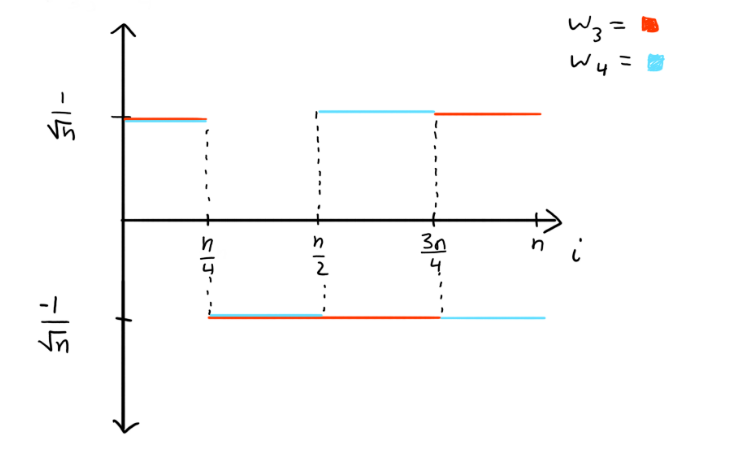
\includegraphics[width=10cm]{graph.png}
	\centering
	\caption{$w_3$ and $w_4$}
	\end{figure}

	\item
	\begin{proof}
	To prove $w_3$ and $w_4$ are in the null space of $M = E[A]$, we show that $Mw_n = 0, n = 3, 4$.
	First, $w_3$.
	\begin{align*}
		Mw_3 &=
		\begin{bmatrix}
			p \cdot \frac{n}{4} - (p \cdot \frac{n}{4} + q \cdot \frac{n}{4}) + q \cdot \frac{n}{4} \\
			\vdots \\
			q \cdot \frac{n}{4} - (q \cdot \frac{n}{4} + p \cdot \frac{n}{4}) + p \cdot \frac{n}{4} \\
			\vdots
		\end{bmatrix} \\
		&=
		\begin{bmatrix}
		0 \\
		0 \\
		\vdots \\
		0
		\end{bmatrix}
	\end{align*}
	Second, $w_4$,
	\begin{align*}
		Mw_3 &=
		\begin{bmatrix}
			p \cdot \frac{n}{4} - p \cdot \frac{n}{4} + q \cdot \frac{n}{4} - q \cdot \frac{n}{4} \\
			\vdots \\
			q \cdot \frac{n}{4} - q \cdot \frac{n}{4} + p \cdot \frac{n}{4} - p \cdot \frac{n}{4} \\
			\vdots
		\end{bmatrix} \\
		&=
		\begin{bmatrix}
		0 \\
		0 \\
		\vdots \\
		0
		\end{bmatrix}
	\end{align*}
	Thus, both $w_3, w_4$ are in the null space of $M$.
	\end{proof}
	\item
	\begin{proof}
	To prove $M = \mu_1 w_1 w_1^T + \mu_2 w_2 w_2^T$, we simply plug in our values. \\
	\textbf{Note: I simplified the formation of M for notational convenience. Recall that M is a block matrix formation and so the different values occur at the half way point in each direction.} \\
	Doing this, we get
	\begin{align*}
	M &= \mu_1 \left( \frac{1}{n}
	\begin{bmatrix}
	1 \\
	1 \\
	\vdots \\
	1 \\
	1 \\
	1 \\
	\vdots \\
	1
	\end{bmatrix}
	\begin{bmatrix}
		1 & 1 & \cdots & 1 & 1 & \cdots
	\end{bmatrix}\right)
	+ \mu_2 \left( \frac{1}{n}
	\begin{bmatrix}
	1 \\
	1 \\
	\vdots \\
	1 \\
	-1 \\
	-1 \\
	\vdots \\
	-1
	\end{bmatrix}
	\begin{bmatrix}
		1 & 1 & \cdots & -1 & -1 & \cdots
	\end{bmatrix} \right) \\
	& = \frac{\mu_1}{n} \left(
	\begin{bmatrix}
	1 & \cdots & 1 \\
	\vdots & \ddots & \vdots \\
	1 & \cdots & 1
	\end{bmatrix} \right)
	+ \frac{\mu_2}{n} \left(
	\begin{bmatrix}
	1 & \cdots & -1 & \cdots \\
	\vdots &  & \vdots \\
	1 & \cdots & -1 & \cdots \\
	-1 & \cdots & 1 & \cdots \\
	\vdots &  & \vdots & \\
	-1 & \cdots & 1 & \cdots
	\end{bmatrix} \right) \\
	&= \frac{1}{2} \left(
	\begin{bmatrix}
	(p + q) + (p - q) & \cdots & (p + q) + (q - p) \\
	\vdots & & \vdots \\
	(p + q) + (q - p) & \cdots & (p + q) + (p - q) \\
	\end{bmatrix}\right) \\
	&= \frac{1}{2} \left(
	\begin{bmatrix}
	2p & \cdots & 2q \\
	\vdots & & \vdots \\
	2q & \cdots & 2p
	\end{bmatrix}\right) \\
	&= M
	\end{align*}
	\end{proof}
	\item In general, we can compute a number (up to the number of communities - given a trivial eigenvector) of eigenvalues and eigenvectors. Then, after inspecting its eigenvector(s), we can separate our communities by looking
	at the sign of the eigenvector(s). This will allow us to cluster certain communities together given that we started with an adjacency matrix.
	\item To find $E[\beta]$ and $Var[\beta]$, we simply calculate directly: \\
	First, $E[\beta]$:
	\begin{align*}
		E[\beta] &= (1 - p)p + (-p)(1-p) \\
		&= \boxed{0}
	\end{align*}
	Second, $Var[\beta]$:
	\begin{align*}
		Var[\beta] &= E[\beta^2] - E^2[\beta] \\
		&= \boxed{(1-p)^2 p + p^2 (1-p)}
	\end{align*}
	\item We can show that $\beta$ is sub-gaussian in a number of ways. One way is that we know bernoulli is sub-gaussian and so translating its values, and so its mean, will not affect its tail distributions as it only affects where they are displaced.
	Thus, it is sub-gaussian. Another way is to use the bound shown here and to see that it satisfies the definition of a sub-gaussian norm, that is
	\begin{equation*}
		\Vert Q \Vert_{\Psi_2} = \inf \{ \lambda > 0, E \left[e^{Q^2/\lambda^2} \right] \le 2\}
	\end{equation*}
	Here, we say
	\begin{equation}
		e^{\frac{\beta^2}{\Vert \beta \Vert_{\Psi_2}^2}} = 2
	\end{equation}
	which implies (via the hint) $1 + (e-1)\frac{\beta^2}{\Vert \beta \Vert_{\Psi_2}^2} = 2$. And so, solving for $\Vert \beta \Vert_{\Psi_2}^2$, we get $\Vert \beta \Vert_{\Psi_2}^2 = (e-1)\beta^2 \le (e-1)$. Finally, this implies that $\Vert \beta \Vert_{\Psi_2} \le \sqrt{e-1}$. Unfortunately, I could not get the bound to be divided in half.
	\item
	\begin{proof}
	Due to how $X$ is constructed, we get
	\begin{align*}
		X &=
		\left[
		\begin{array}{c|c}
			\beta(p) & \beta(q) \\
			\hline
			\beta(q) & \beta(p)
		\end{array}
		\right]
	\end{align*}
	Thus,
	\begin{align*}
		\left[
		\begin{array}{c|c}
			E[\beta(p)] & E[\beta(q)] \\
			\hline
			E[\beta(q)] & E[\beta(p)]
		\end{array}
		\right]
	&= \left[
		\begin{array}{c|c}
			0 & 0 \\
			\hline
			0 & 0
		\end{array}
		\right]\\
	&=
	\begin{bmatrix}
	0 & \cdots & 0 \\
	\vdots & \ddots & \vdots \\
	0 & \cdots & 0
	\end{bmatrix}_{n \times n}
	\end{align*}
	\end{proof}
	\item
	\begin{proof} Recall that if our matrix, $A$, is square, that is $n = m$, then we can say
	$\Vert A \Vert = \vert \lambda_1 \vert$. Thus, We have $E[\Vert X \Vert] = E[\vert \lambda_1 \vert].$ And so, from the textbook,
	we can use corollary 4.4.8 to say
	\begin{equation}
		\Vert X \Vert \le c_1K(\sqrt{n} + t)
	\end{equation}
	And so,
	\begin{equation}
		E[\Vert X \Vert] \le c_1 \sqrt{n}
	\end{equation}
	since $Var[X] \le 1$ and $t$ goes away on expectation. Thus, we have
		\begin{equation}
		E[\Vert X \Vert] = E[\vert \lambda_1 \vert] \le c_1 \sqrt{n}
	\end{equation}
	\end{proof}
	\item
	\begin{proof}
	Using Weyl-Lidskii Theorem, and letting $A = M, E = X$, we can say for $\lambda_i, i = 1,2$,
	\begin{equation}
	\vert \lambda_1 (M) - \lambda_1 (M + X) \vert \le \Vert X \Vert
	\end{equation}
	Using our previous answers, we can use the fact that $\Vert X \Vert \sim \sqrt{n}$ and $\lambda_i \sim n$, as well as $A = M + X$, to deduce
	\begin{align*}
		\vert \lambda_i (M) - \lambda_i (M + X) \vert &\le \Vert X \Vert \\
		\implies -c\sqrt{n} + \lambda_i(M) &\le \lambda_i(A) \le \lambda_i(M) + c\sqrt{n} \\
		\implies \lambda_i(M) &\le \lambda_i(A) \le \lambda_i(M) \hspace{0.2cm}\text{(for large $n$, since $n > \sqrt{n}$)}
	\end{align*}
	Thus, by a similar proof of squeeze theorem, the eigenvalues of $A$ approach the eigenvalues of $E[A] = M$. Note, we are considering non-trivial eigenvalues
	as our high-dimensional matrix is low rank ($r = 2$). Additionally, the bounds on $p$ and $q$ allow for our eigenvalue to not overlap between our first and second eigenvalues on their edge of bounding.
	This then satisfies the premise of the theorem that they are ordered for any value of $n$ and so can be considered in full.
	\end{proof}
\end{enumerate}
\begin{center}
	\boxed{{\textbf{| END |}}}
\end{center}
\end{document}